La diferencia fundamental entre un FF-D implementado con \textit{transmission gates} (TG) y uno que no los utiliza reside en cómo se controla la transferencia y el aislamiento de la información en cada latch.

En la versión con  TG, el paso de la señal se realiza a través de interruptores bidireccionales compuestos por un NMOS y un PMOS en paralelo. Esta configuración permite una conducción prácticamente ideal de ambos niveles lógicos (‘0’ y ‘1’), evitando degradaciones de amplitud. Además, el nodo interno queda efectivamente aislado cuando el switch está abierto, lo que asegura que cada latch capture y mantenga el dato de manera robusta, incluso frente a flancos de clock no ideales o variaciones en la entrada.

Por el contrario, cuando se emplean transistores individuales gobernados por el clock, la conducción se vuelve inherentemente asimétrica: el NMOS introduce una caída en el nivel alto, mientras que el PMOS degrada el nivel bajo. A esto se suma un aislamiento menos eficiente del nodo interno, incrementando la susceptibilidad a corrientes de fuga, ruido y posibles solapamientos en las fases del clock. Como consecuencia, esta implementación presenta menor integridad de señal, pudiendo generar glitches, pérdidas del dato almacenado o incluso la propagación parcial de la entrada en condiciones en las que debería mantenerse estable.

\begin{figure}[H]
    \centering
    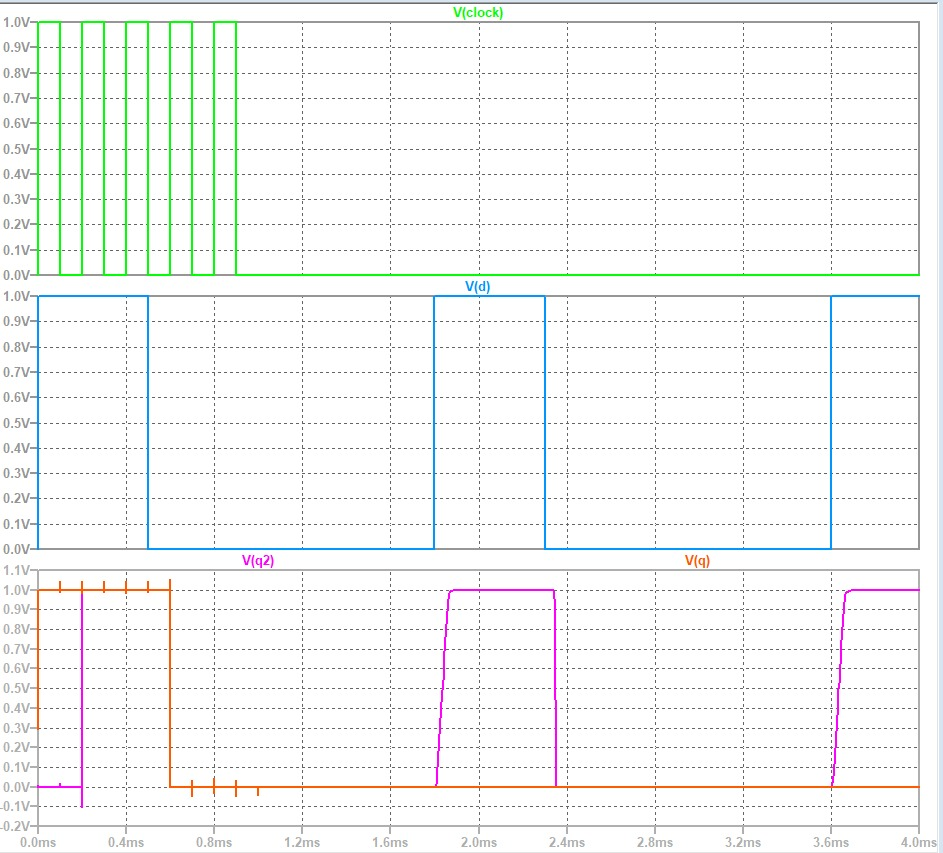
\includegraphics[width=0.8\textwidth]{Imagenes/FFMalo.jpeg}
    \caption{Comparación entre FF-D con y sin TG}
    \label{fig:FFD_comparison}
\end{figure}


Donde $V_{d}$ corresponde a la señal de entrada, $V_{(q)}$ a la salida del circuito implementado con TG, y $V_{(q2)}$ a la salida del circuito que no los utiliza.

Si se considera un clock con únicamente dos pulsos, se espera que la implementación con TG sea capaz de mantener (hold) el valor almacenado, mientras que la implementación sin estos dispositivos no debería lograrlo. Los resultados obtenidos en la simulación fueron los siguientes:

\begin{figure}[H]
    \centering
    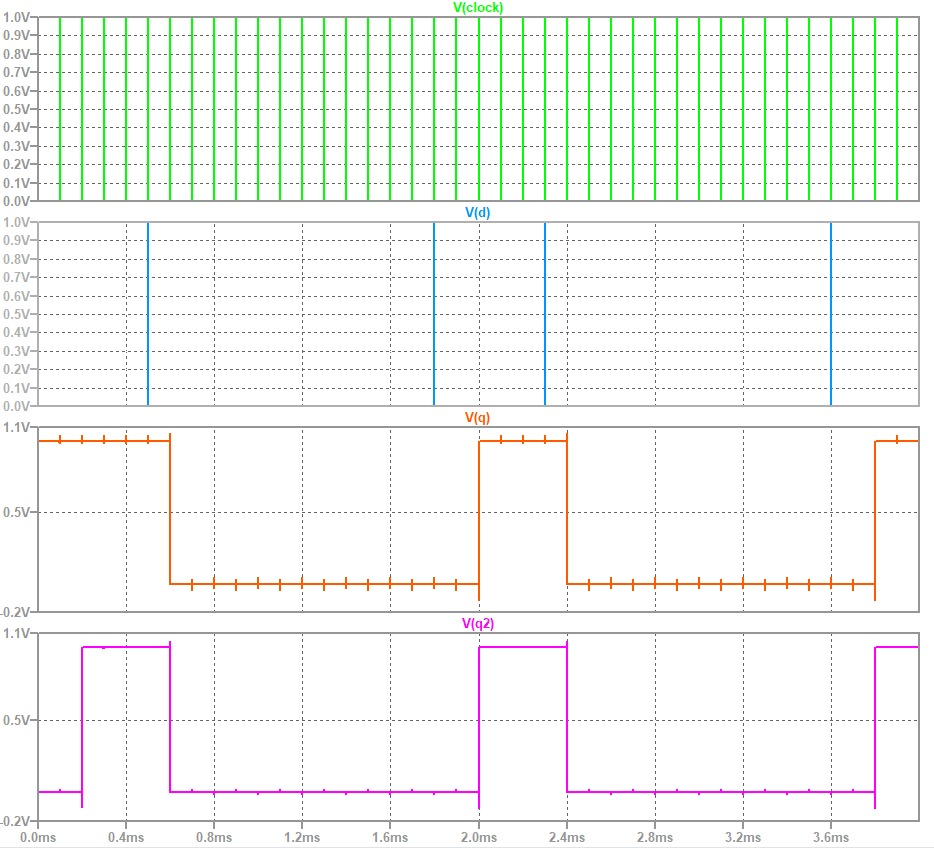
\includegraphics[width=0.8\textwidth]{Imagenes/FFBueno.jpeg}
    \caption{Simulación de FF-D con y sin TG}
    \label{fig:FFD_simulation}
\end{figure}

Cuando el clock es periódico, ambos circuitos presentan un comportamiento similar, ya que las pequeñas degradaciones de nivel lógico quedan compensadas y no afectan significativamente la conmutación. Sin embargo, cuando el clock deja de alternar, como en la simulación realizada, se pone en evidencia la diferencia estructural: en ausencia de transistores que actúen como TG, el latch no logra mantener un aislamiento adecuado y la salida pierde el dato almacenado, mientras que la implementación con TG conserva el valor sin inconvenientes.

